\documentclass[]{article}

% Imported Packages
%------------------------------------------------------------------------------
\usepackage{amssymb}
\usepackage{amstext}
\usepackage{amsthm}
\usepackage{amsmath}
\usepackage{enumerate}
\usepackage{fancyhdr}
\usepackage[margin=1in]{geometry}
\usepackage{graphicx}
\usepackage{extarrows}
\usepackage{setspace}
%------------------------------------------------------------------------------

% Header and Footer
%------------------------------------------------------------------------------
\pagestyle{plain}  
\renewcommand\headrulewidth{0.4pt}                                      
\renewcommand\footrulewidth{0.4pt}                                    
%------------------------------------------------------------------------------

% Title Details
%------------------------------------------------------------------------------
\title{Deliverable \#3 Template}
\author{SE 3A04: Software Design II -- Large System Design}
\date{}                               
%------------------------------------------------------------------------------

% Document
%------------------------------------------------------------------------------
\begin{document}

\maketitle	

\section{Introduction}
\label{sec:introduction}
% Begin Section

This section provides a brief overview of the entire document.

\subsection{Purpose}
\label{sub:purpose}

The purpose of this document is to give an outline of the detailed design of the AudioVal.ly system; including a description of the system's behaviour, interactions of the subsystems and components, and finally a detailed outline of all the classes that will compose this system as a whole.

The target audience for this document are the stakeholders (Dr. Ridha Khedri, Spencer Deevy and Andrew Le Clair ), and any current or future architects, designers and developers of this project.

\subsection{System Description}
\label{sub:system_description}

The AudioVal.ly application is intended to identify different music genres of music. The primary interface between the user and the software system is through a device running the Android
operating system. This document defines the way in which the users will be expected to interact with the system and how the application will be decomposed into smaller subsystems to reduce the complexity and improve the maintainability and flexibility of this system.

Specifically, the users of this system (application) are expected to perform a set of events that will prompt the system to react. The decomposition will then show how the subsystems will communicate among one another in order to efficiently distribute the work and perform the required actions in response to the user's actions.


\subsection{Overview}
\label{sub:overview}
The remainder of this document is organized into 3 sections: State Charts for Controller Classes -- defining the behaviour of the controller classes, Sequence Diagrams -- outlining the sequence of interactions between different subsystems for various business events, and Detailed Class Diagram -- specifying the classes that will compose the system, the relations between
classes and the methods each class provides. Each section uses appropriate UML diagrams to describe and document the design details.

\newpage
\section{State Charts for Controller Classes}
\label{sec:state_charts_for_controller_classes}
% Begin Section
This section provides a state chart for each controller class for the application.
% End Section
\begin{center}
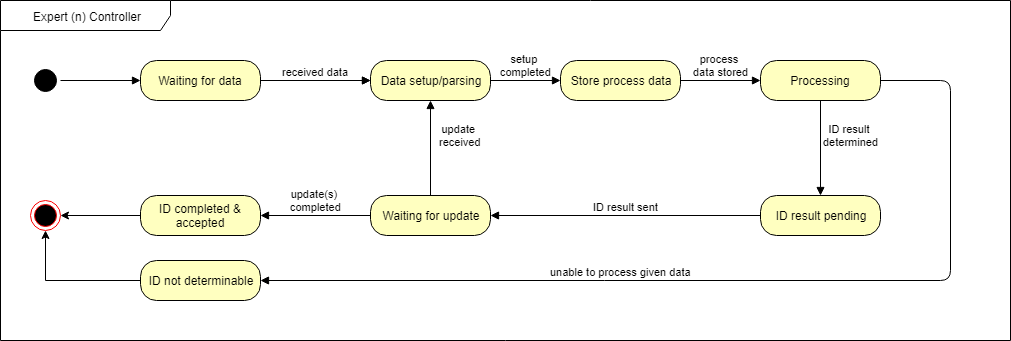
\includegraphics[scale=0.5]{ExpertnController}
\end{center}
\begin{center}
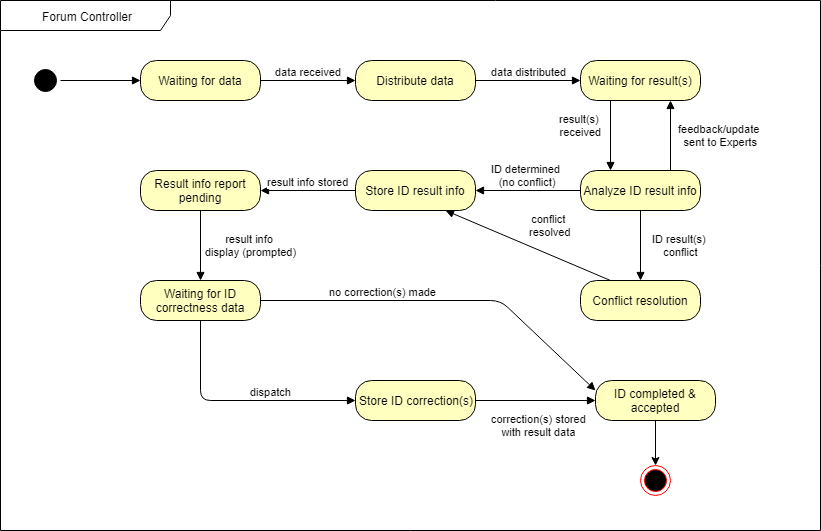
\includegraphics[scale=0.5]{ForumController}
\end{center}
\begin{center}
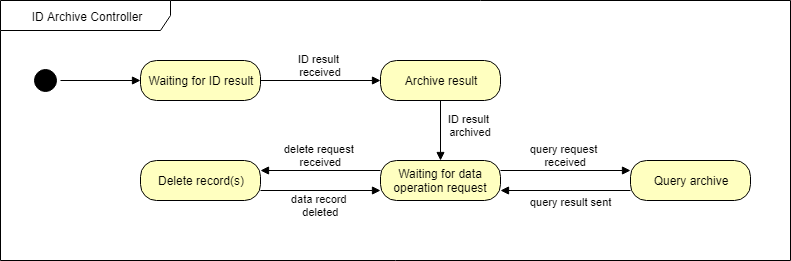
\includegraphics[scale=0.5]{IDArchiveController}
\end{center}
\begin{center}
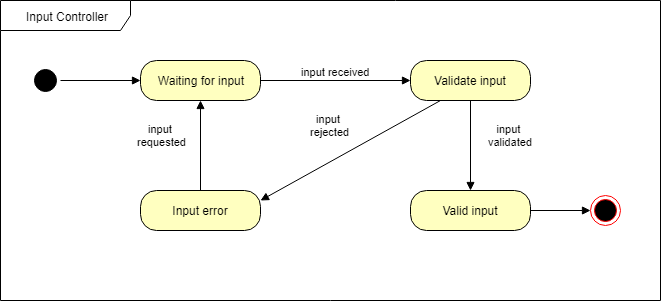
\includegraphics[scale=0.5]{InputController}
\end{center}
\begin{center}
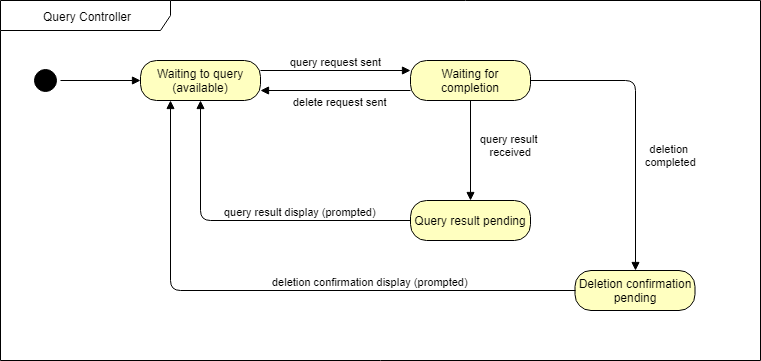
\includegraphics[scale=0.5]{QueryController}
\end{center}
\begin{center}
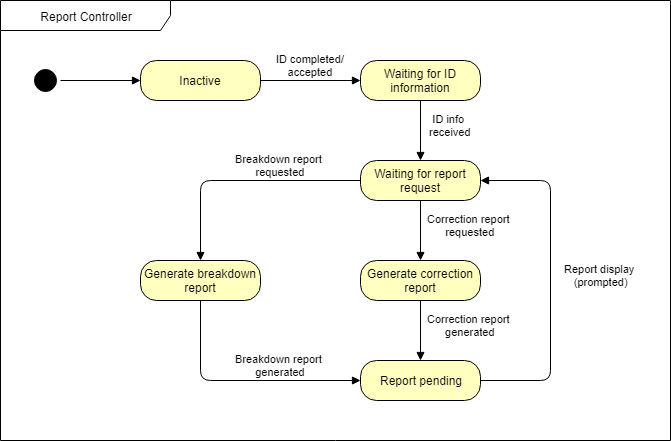
\includegraphics[scale=0.5]{ReportController}
\end{center}

\newpage
\section{Sequence Diagrams}
\label{sec:sequence_diagrams}
% Begin Section
This section provides a sequence diagram for each use case of the application.
% End Section
\\
\begin{center}
	Correct An Identification
  \makebox[\textwidth]{\includegraphics[width=\linewidth]{UseCaseCorrectAnIdentification1}}
  \makebox[\textwidth]{\includegraphics[width=\linewidth]{UseCaseCorrectAnIdentification2}}
	\newpage
	Delete An Identification
  \makebox[\textwidth]{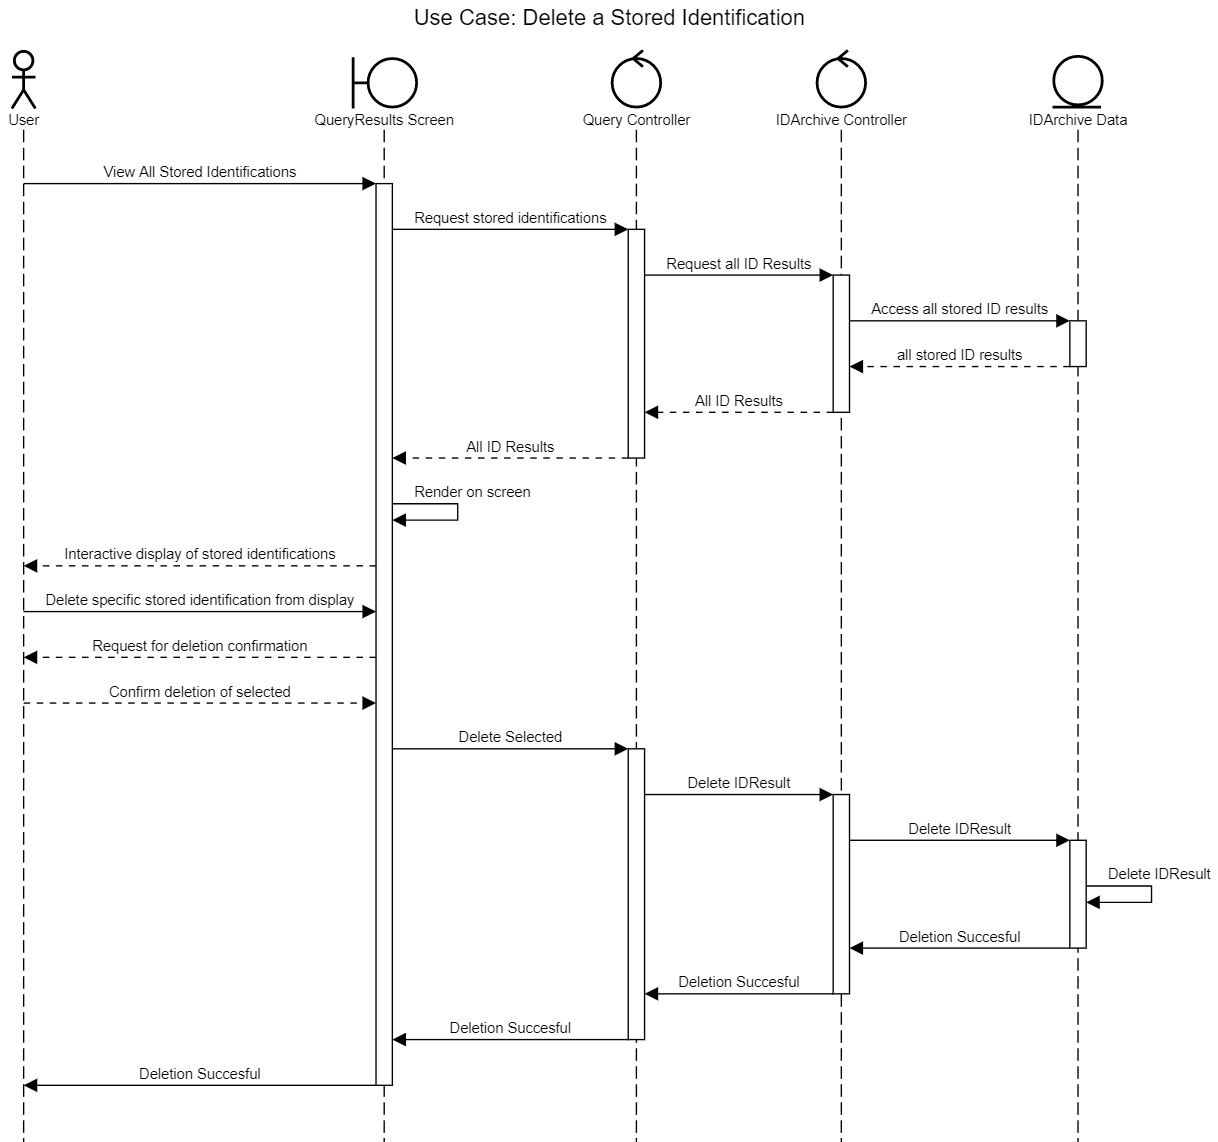
\includegraphics[width=\linewidth]{UseCaseDeleteaStoredIdentification}}
	\newpage
	Identify A Song/Music
  \makebox[\textwidth]{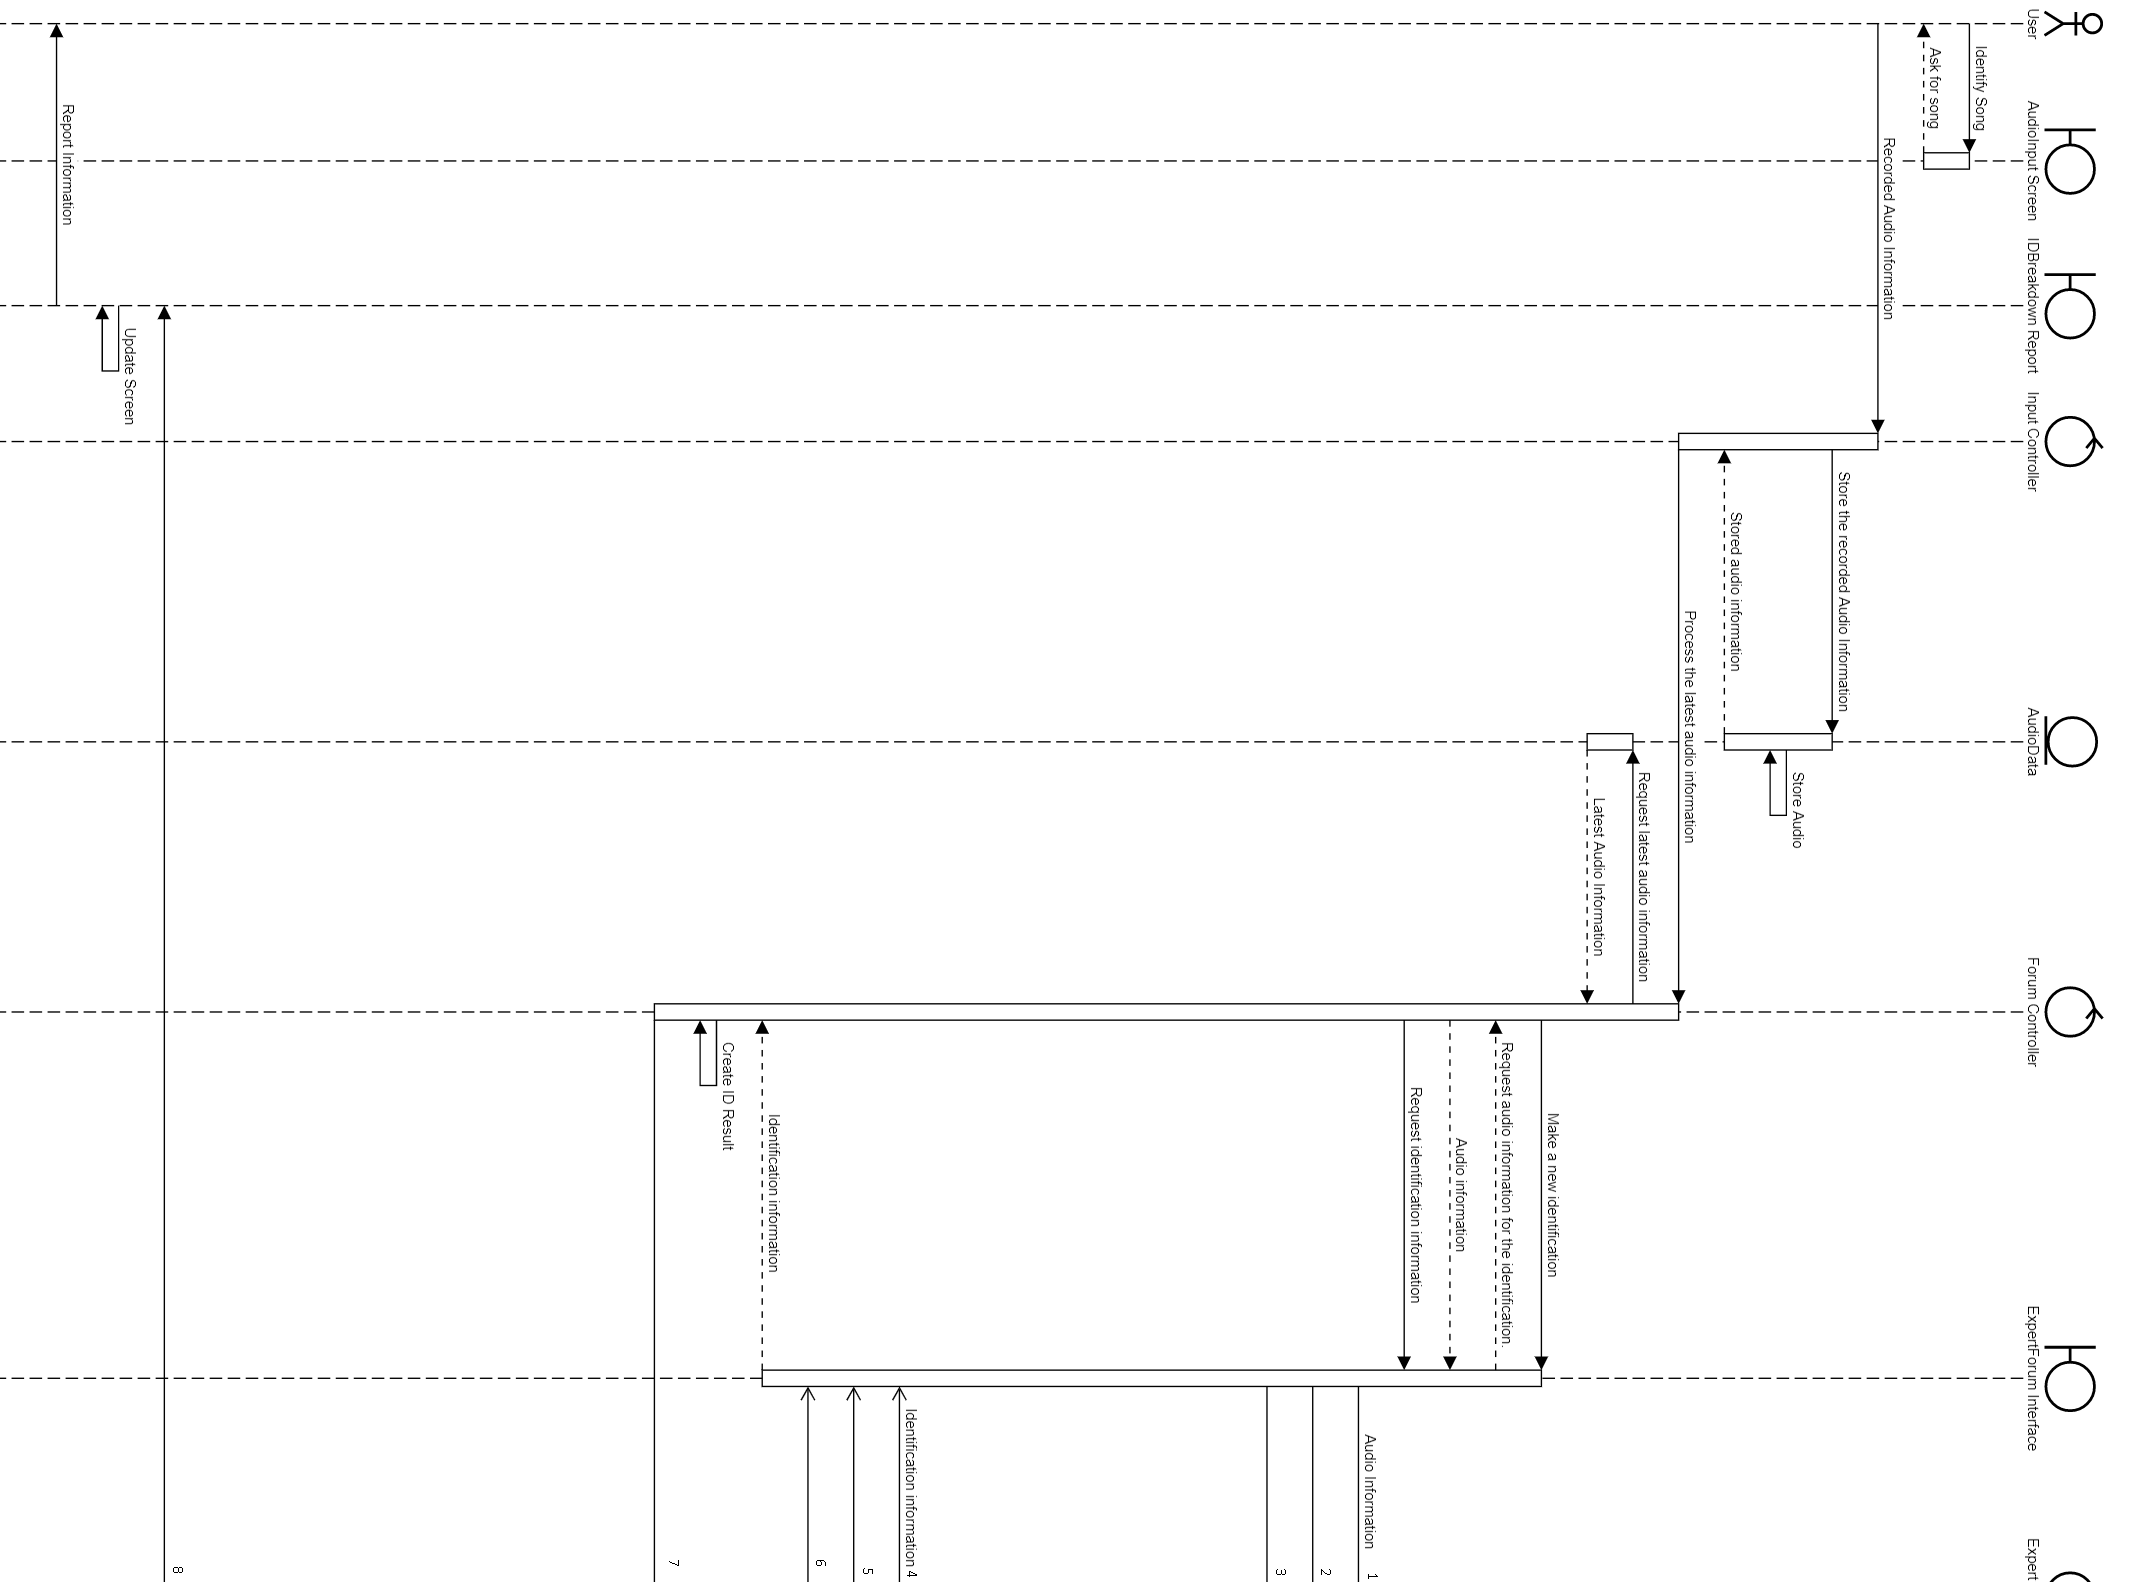
\includegraphics[width=\linewidth]{UseCaseIdentifyASongMusic1}}
  \makebox[\textwidth]{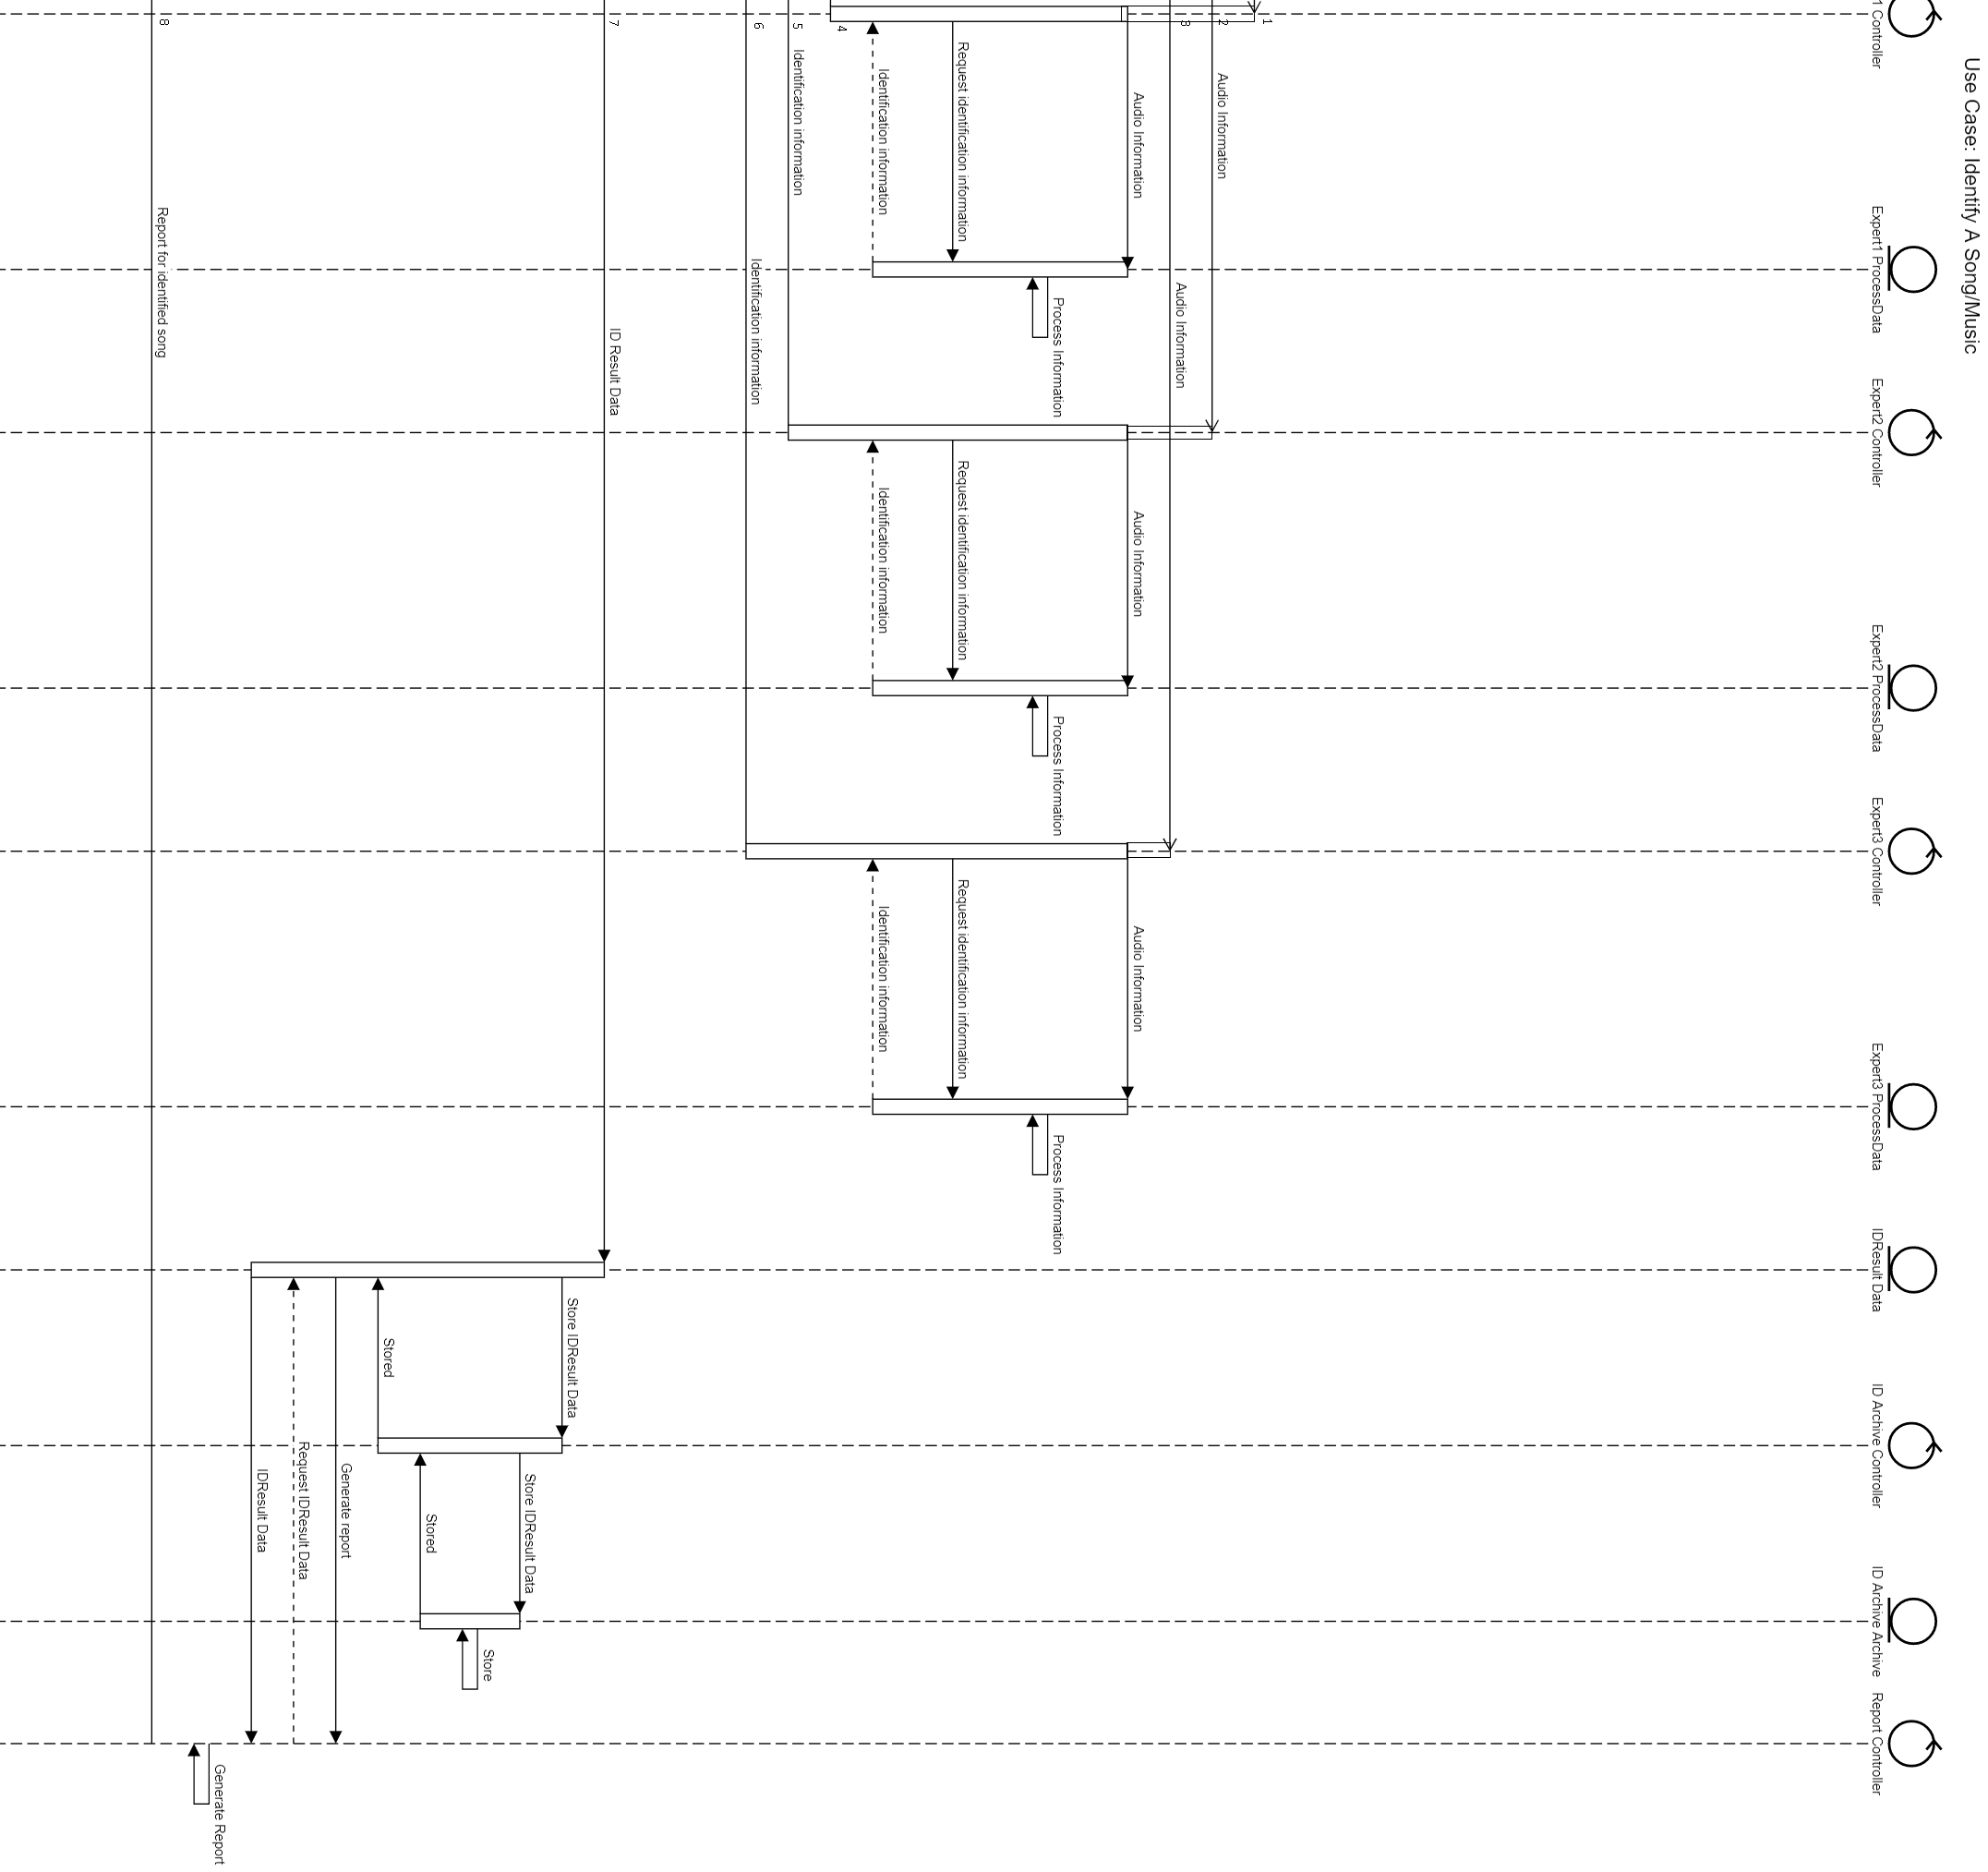
\includegraphics[width=\linewidth]{UseCaseIdentifyASongMusic2}}
	\newpage
	Re-evaluate An Identification
  \makebox[\textwidth]{\includegraphics[width=\linewidth]{UseCaseReevaluateAnIdentification1}}
  \makebox[\textwidth]{\includegraphics[width=\linewidth]{UseCaseReevaluateAnIdentification2}}
	\newpage
	Store An Identification
  \makebox[\textwidth]{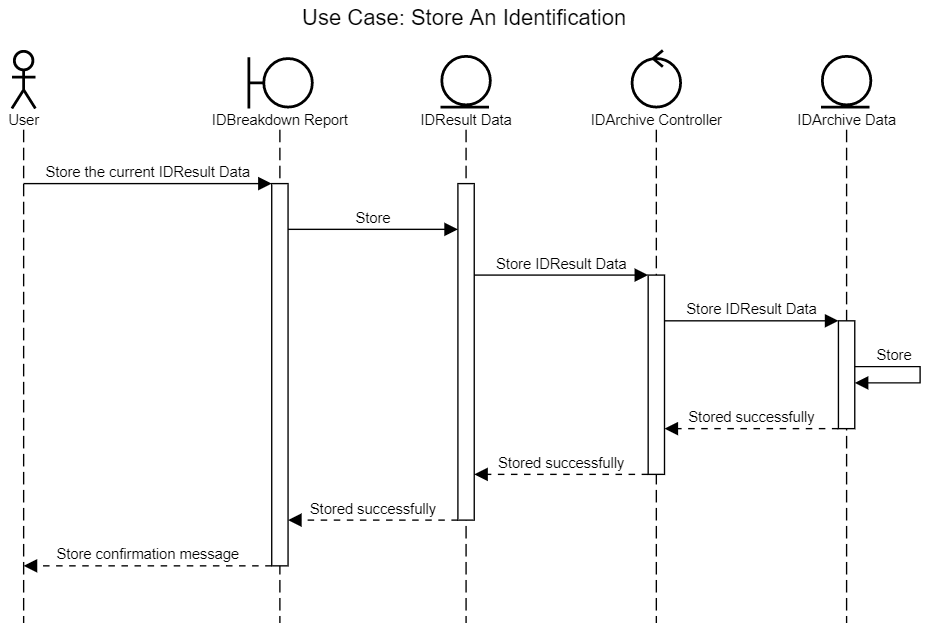
\includegraphics[width=\linewidth]{UseCaseStoreAnIdentification}}
	\newpage
	View All Stored Identifications
  \makebox[\textwidth]{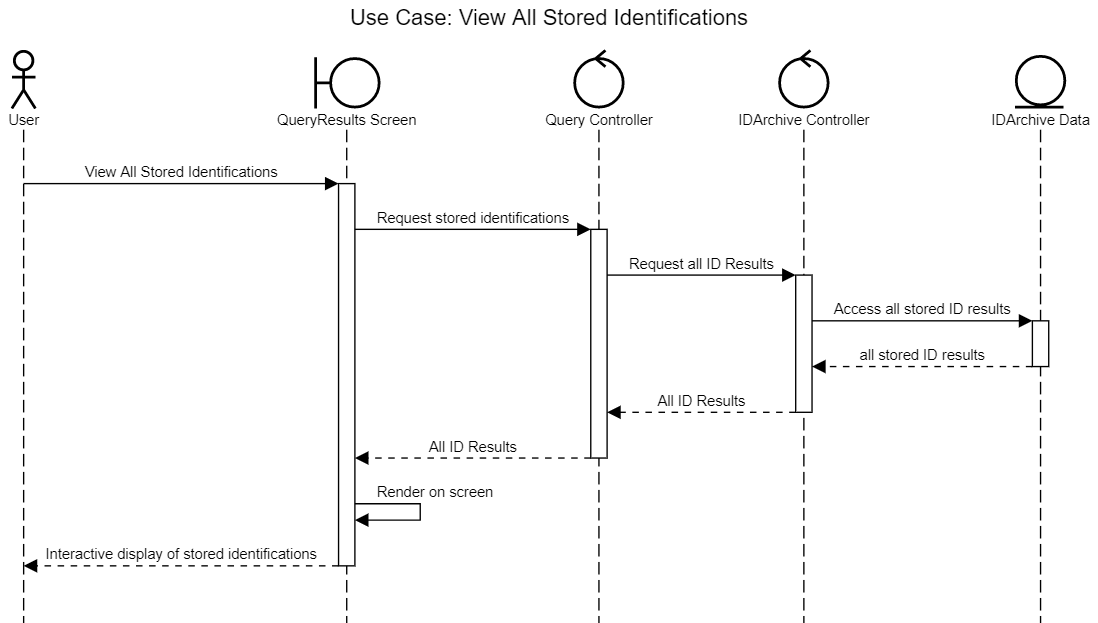
\includegraphics[width=\linewidth]{UseCaseViewAllStoredIdentifications}}
	\newpage
	View A Specific Stored Identification
  \makebox[\textwidth]{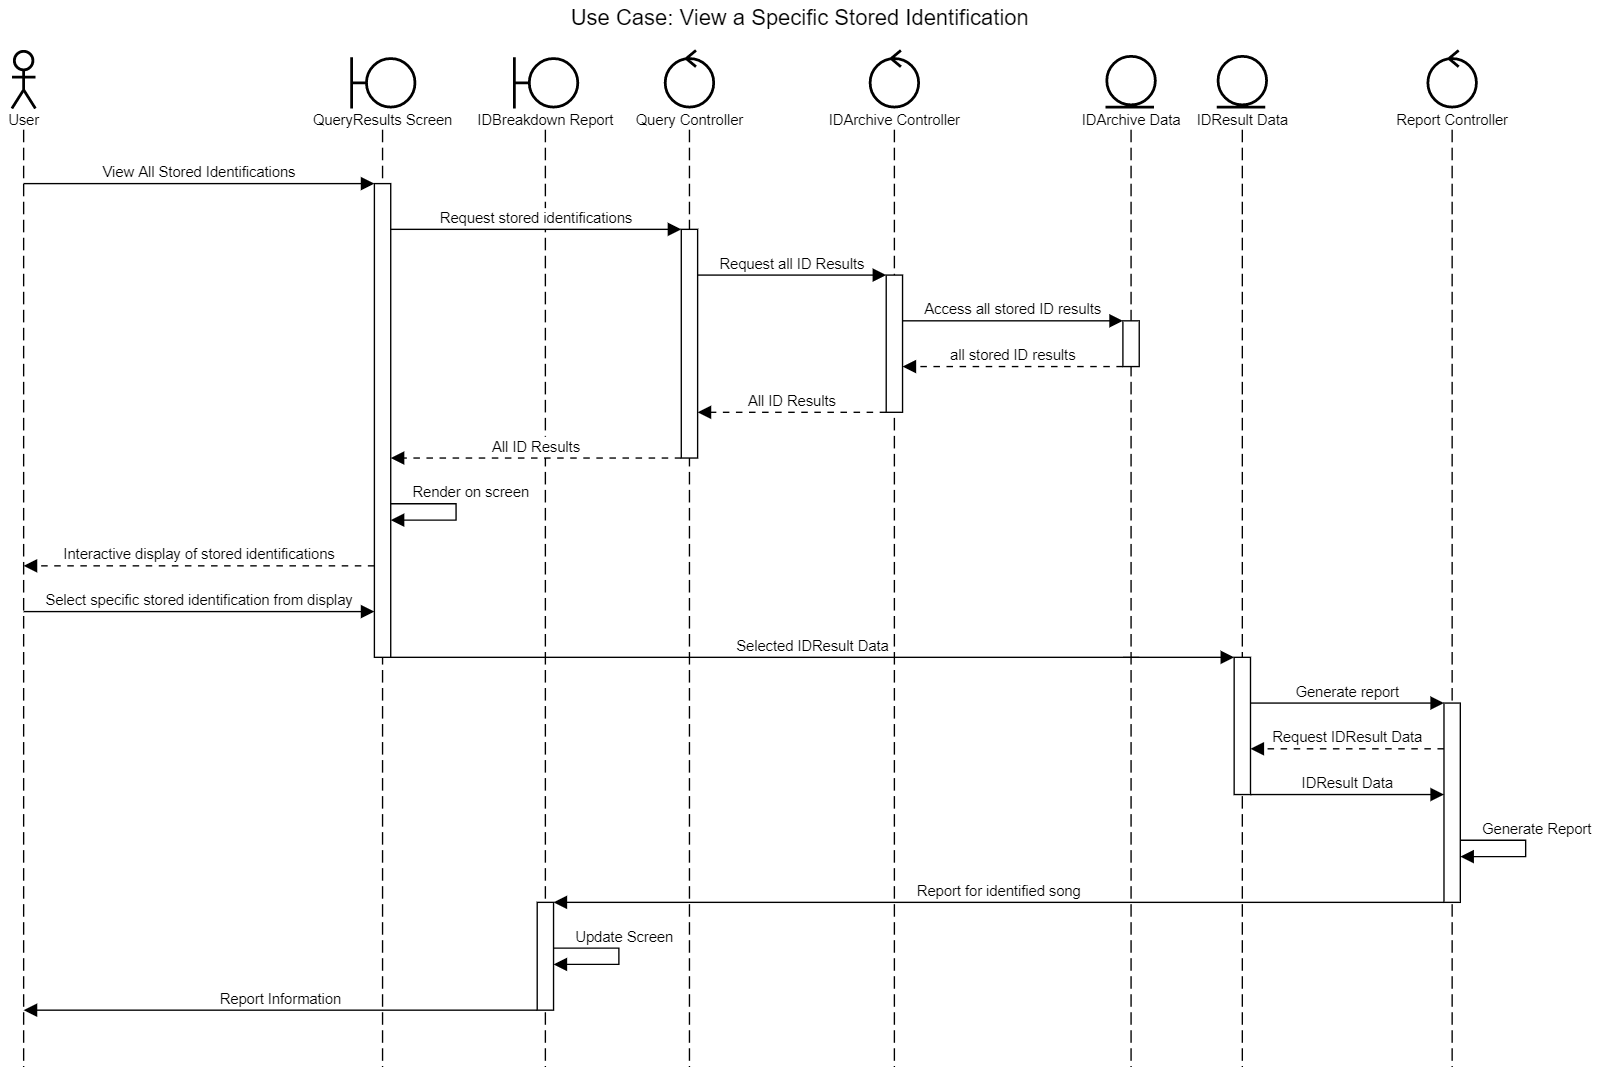
\includegraphics[width=\linewidth]{UseCaseViewASpecificStoredIdentification}}
	\newpage
	View Identification Rationale
  \makebox[\textwidth]{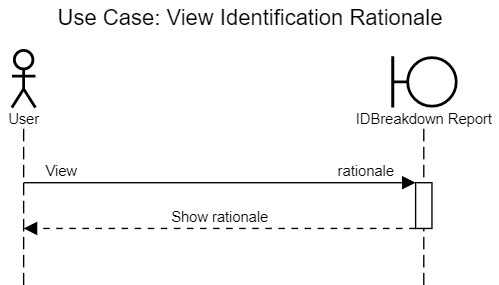
\includegraphics[width=\linewidth]{UseCaseViewIdentificationRationale}}
\end{center}

\section{Detailed Class Diagram}
\label{sec:detailed_class_diagram}
% Begin Section
This section provides a detailed class diagram for the application.
% End Section

\appendix
\section{Division of Labour}
\label{sec:division_of_labour}
% Begin Section
% End Section

\newpage
\section{Division of Labour}
\label{sec:division_of_labour}
\begin{center}
\large
			\begin{tabular}{l|c}
				Work Completed   & Contributors \\\hline
				Production Conceptualisation &Team 11 \\
				HLAD Section 1 : Introduction & Puru Jetly \\
				HLAD Section 2 : State Charts for Controllers  & Baltej Toor \\
				HLAD Section 3 : Sequence Diagrams  & Brandon Roberts, Corey Szeto \\
				HLAD Section 4 : Detailed Class Diagrams & Jiahong Dong \\
				HLAD Final Review + Latex  & Brandon Roberts, Baltej Toor \\
			\end{tabular}
			\vspace{0.1in}
\huge Signatures
\end{center}
			\vspace{0.3in}
\large
			\begin{tabular}{l|r}
			\vspace{1in}
				Baltej Toor  & \underline{\hspace{8cm}} \\
			\vspace{1in}
				Brandon Roberts   & \underline{\hspace{8cm}} \\
			\vspace{1in}
				Corey Szeto  & \underline{\hspace{8cm}} \\
			\vspace{1in}
				Jiahong Dong   & \underline{\hspace{8cm}} \\
			\vspace{1in}
				Puru Jetly   & \underline{\hspace{8cm}} \\
			\end{tabular}


\end{document}
%------------------------------------------------------------------------------